\fancyhead[C]{Section 16.2}
	\fancyhead[R]{\daytwentytwo}

\iftoggle{questions}{
\begin{center}{\large \textbf{Math 2551 Worksheet: Vector Line Integrals}}
\end{center}

\begin{enumerate}
	
	\item Consider the vector field $\bF$ (thin arrows) and and let $\bT$ denote the unit tangent vector to the directed curves shown below (denoted with thick arrows). Determine whether \[ \int_C \bF\cdot\bT\ ds\] is positive, negative, or zero for each directed curve $C$.  In other words, determine whether the \textit{work} done by the vector field on each curve is positive, negative, or zero.
	
	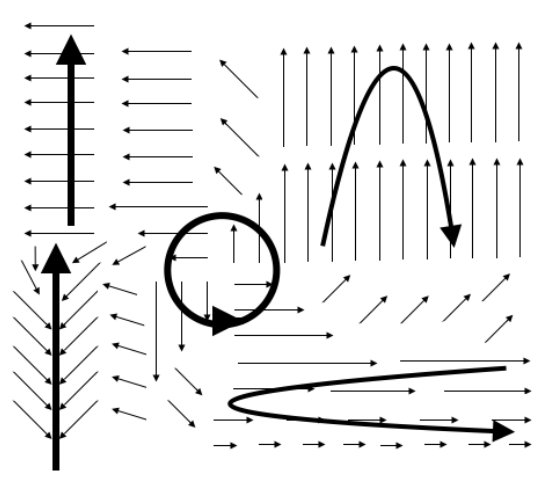
\includegraphics[scale=0.5]{16_2pic.png}
	
	
	\item Evaluate $\int_C (2x -y)\bi\cdot\ d\br$ where $C$ is parameterized by 
	$\br(t) = (t^2)\bi+(3t-2)\bj$ , $t \in [0,1]$.\\
	
	\item Find the work done by the force $\bF= xy \bi +(y-x) \bj$ over the straight line from $(1,1)$ to $(2,3)$.\\
	
	\item Consider the closed curve $C$ consisting of a semicircle and a straight line segment as follow:
	\[
	\br_1(t)=(2 \cos t)\bi+(2 \sin t)\bj, \ t \in [0,\pi], \qquad \br_2(t)=t\bi, \ t\in [-2,2]
	\]
	Let the vector field $\bF$ be given by 
	\[
	\bF(x,y) = -y^2 \bi + x^2 \bj.
	\]
	Find the circulation of $\bF$ around $C$ and the flux of $\bF$ across $C$. 
	%%
	
	\item Give an example of a non-trivial force field $\bF$ (not the zero vector at all points) and a non-trivial path $\br(t)$ (not the stationary path at a point $P$) for which the total work done moving along the path is zero.
\end{enumerate}
}{}

\iftoggle{answers}{
\begin{center}{\large \textbf{Math 2551 Worksheet Answers: Vector Line Integrals}}
\end{center}
\begin{enumerate}
	\item Top left: 0 \\
	Bottom left: Negative \\
	Center: Positive \\
	Top right: 0\\
	Bottom right: Negative
	
	
	\item 1
	
	\item $\dfrac{25}{6}$
	
	\item Circulation: $\dfrac{32}{3}$\\
	Flux: 0
	
	\item Many possible examples: the top left and top right examples from 1), $\nabla f$ for any $f$ together with a closed curve $\br$, any example where $\bF\cdot \br'(t)=0$, i.e. the field and curve are orthogonal, and more.
\end{enumerate}
}{}
\iftoggle{solutions}
{
Solutions go here in the same format.
}{}
